\EnglishSourceFrame{GELFAND-P001445}{30}
Construct a complex from these data
\begin{equation*}
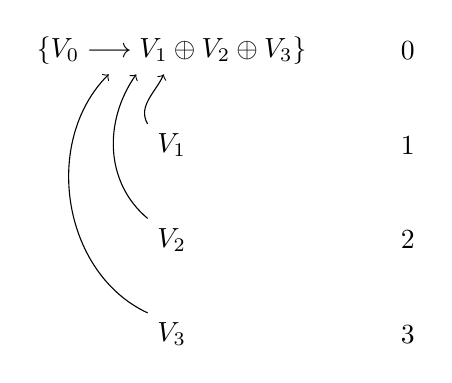
\begin{tikzpicture}
\node (c) at (0,0) {$\{V_0\longrightarrow V_1\oplus V_2\oplus V_3\}$};
\node (v1) at (0,-1.2) {$V_1$};
\node (v2) at (0,-2.4) {$V_2$};
\node (v3) at (0,-3.6) {$V_3$};
\node at (3,0) {$0$};
\node at (3,-1.2) {$1$};
\node at (3,-2.4) {$2$};
\node at (3,-3.6) {$3$};
\draw[->] (v1.north west) to[out=120,in=245] (-0.1,-0.3);
\draw[->] (v2.north west) to[out=140,in=235] (-0.45,-0.3);
\draw[->] (v3.north west) to[out=155,in=225] (-0.8,-0.3);
\end{tikzpicture}
\end{equation*}
This is an object of the derived category (of representations of the quiver)
\begin{equation*}
\begin{tikzcd}[column sep=large,row sep=small]
 & 1 \arrow[dl]\\
0 & 2 \arrow[l]\\
 & 3 \arrow[ul]
\end{tikzcd}
\end{equation*}
The quotient in the ordinary category should be replaced by the map itself
(the complex).

\EnglishUnclear{GELFAND-P001445}{bottom-name}{Parti\ldots [surname illegible]}
poses and solves the question of when the derived category coincides with this one
(for $3$, but not for $4$).

\EnglishSourceFrame{GELFAND-P001446}{unlabelled}
\underline{23. III. 88}\qquad \underline{Gelfand's seminar.}

\underline{A. Zelevinsky.}\qquad \underline{Matroids and Hall's theorem}

\underline{I.M.G.}

Matroid. [Above the following word, crossed out:
\EnglishUnclear{GELFAND-P001446}{intro-deletion}{illegible cancelled signs}.]
\underline{Example:} linearly independent systems of vectors.
\begin{equation*}
M_1,M_2\text{ are sets},\qquad \varphi\subset M_1\times M_2
\end{equation*}
(a relation)

Suppose $M_1$ has a matroid structure.

How can a matroid structure be introduced on $M_2$?
\begin{equation*}
A\subset M_2,\qquad \pi_1\bigl(\pi_2^{-1}(A)\cap\varphi\bigr)
\text{ is a set}.
\end{equation*}
[Below the dash, crossed out:
\EnglishUnclear{GELFAND-P001446}{image-set-deletion}{illegible}.]

The rank of the set $A$ is defined

$1^{\circ}$. \underline{Rado's theorem}
\begin{equation*}
r_{M_2}(A)=\min_{B\subset A}
\bigl(r_{M_1}(\varphi(B))+|A-B|\bigr),\qquad A\subset M_2.
\end{equation*}
$2^{\circ}$. \underline{Hall's theorem} $\equiv$
[Inserted above the surname:
\EnglishUnclear{GELFAND-P001446}{hall-insertion}{F. [Cyrillic initial] / $\varphi$}.]

[Crossed out on the left:
\EnglishUnclear{GELFAND-P001446}{hall-left-deletion}{illegible}.]
\underline{The marriage problem}:
[Inserted above the line: a set $M$ of grooms,
$\operatorname{Card}M\geq\operatorname{Card}N$.]

If there are [above $N$, inserted: a set of] $N$ brides and
[crossed out: $M\geq N$ grooms], each groom $m\in M$
likes brides $A(m)\subset N$; moreover,
[crossed out: $\forall A\subset N$] $\forall$ subsets
$K\subset N$,
[Above the formula, crossed out:
\EnglishUnclear{GELFAND-P001446}{card-deletion}{an illegible sign}.]
\begin{equation*}
\operatorname{Card}\left(\bigcup_{n\in K}B(n)\right)
\geq \operatorname{Card}K.
\end{equation*}

\EnglishSourceFrame{GELFAND-P001447}{37}
(Here $B(n)\subset M$;
[below $B(n)$, linked by an equals sign:]
the set of grooms who like $n$, i.e.
\begin{equation*}
B(n)=
\{m:\ n\in A(m)\}
\end{equation*}
[After $=$, crossed out:
\EnglishUnclear{GELFAND-P001447}{top-b-deletion}{an illegible sign}.])

Then $\exists$ a one-to-one choice
[crossed out: \EnglishUnclear{GELFAND-P001447}{choice-deletion}{illegible}]:
a map $f:N\longrightarrow M$, for which
\begin{equation*}
f(n)\subset B(n)\qquad \forall n.
\end{equation*}
\EnglishUnclear{GELFAND-P001447}{hall-membership}{The source has $f(n)\subset B(n)$.}

[Crossed-out line: Hall's theorem\quad $\varphi$ is a relation.]

[Crossed out: Theor.]
There is a proof containing an algorithm.

\underline{Reduction to Rado's theorem}: all subsets of $N$ must be declared independent.

$2^{\circ}\Rightarrow 3^{\circ}$. \underline{Birkhoff's theorem.}

Hall's theorem implies that, given a subgroup $H\subset G$
[below $G$: finite group],
$\exists$ a system of common representatives of the left and right cosets.

\underline{I.M.G.} There are several famous problems whose senselessness
is obvious to everyone.

\underline{Example.} 1) \underline{The parallel axiom}

(why precisely this one?)

[Below this line:]
\EnglishUnclear{GELFAND-P001447}{parallelism-note}{worked on them [two possible source pronoun forms]}

[To the right of the first two lines, beyond a vertical line:]
$\Rightarrow$ non-Euclidean geometry.

2) \underline{Trisection of an angle} and squaring the circle.
\begin{equation*}
\text{Trisection of an angle}\ \Downarrow\ \text{Galois theory}
\end{equation*}
3) \underline{Fermat's theorem}
\begin{equation*}
\Downarrow
\end{equation*}
the theory of [crossed out:
\EnglishUnclear{GELFAND-P001447}{ideals-deletion}{an illegible letter}]
ideals (Kummer) and algebraic geometry.
[On the right, beyond a vertical line:] Faltings's work.

4) \underline{The $4$-colour problem}
\begin{equation*}
\Downarrow\quad ?
\end{equation*}
These works should be examined.

5) \underline{The Riemann hypothesis}

\EnglishSourceFrame{GELFAND-P001448}{unlabelled}
\underline{A. Rudakov.}\quad
\underline{Vector bundles, braid groups and Diophantine equations.}

$1^{\circ}$. On $\mathbb{P}^{2}\ (= \mathbb{C}\mathbb{P}^{2})$

consider vector bundles (or coherent sheaves)
\begin{equation*}
E_1,\ E_2,\ E_3 \tag{1}
\end{equation*}
[After $E_1$, crossed out:
\EnglishUnclear{GELFAND-P001448}{triple-deletion}{illegible signs}.]
\begin{equation*}
\begin{gathered}
\operatorname{Ext}^{k}(E_j,E_i)=0,\quad j>i,\quad k=0,1,2,\\
\operatorname{Ext}^{k}(E_i,E_i)=
\begin{cases}
0,& k>0,\\
\mathbb{C},& k=0.
\end{cases}
\end{gathered}
\tag{2}
\end{equation*}
[Before $k=0,1,2$, crossed out:
\EnglishUnclear{GELFAND-P001448}{ext-deletion}{an illegible sign}.]

Such bundles exist, and if $\dim E_j=x_j$, then
\begin{equation*}
x_1^2+x_2^2+x_3^2=3x_1x_2x_3
\qquad\text{(Markov equation)} \tag{3}
\end{equation*}
(and all [inserted above: integer] solutions are realized in this way!)

The braid group acts on the tuples [inserted above: (1) (there are countably many of them)],
and all tuples (1) constitute one orbit!

$2^{\circ}$.
\begin{equation*}
Q=\mathbb{P}^{1}\times\mathbb{P}^{1}.
\end{equation*}
[After $Q=$, crossed out:
\EnglishUnclear{GELFAND-P001448}{quadric-deletion}{an illegible sign}.]

Then take 4 bundles $E_1,E_2,E_3,E_4$
with the same conditions (2); the braid group acts here too.

Instead of (3), a system of Diophantine equations appears
(but the correspondence is in one direction; it is not proved that all solutions arise).
This is something like a root system in which the braid group appears
in place of the Weyl group.

$3^{\circ}$. On $\mathbb{P}^{n}$ one can consider bundles
\begin{equation*}
E_1,E_2,\ldots,E_{n+1}\qquad\text{with conditions (2)}
\end{equation*}
and an action of the braid group appears again.

\underline{M. Kapranov}: on the braid group action.

\underline{I.M.G.}

Solvable and unsolvable classification problems.

No parameters $\Rightarrow$ classifiable (manual)

1 parameter $\Rightarrow$
[crossed out: \EnglishUnclear{GELFAND-P001448}{classification-correction}{manual (\ldots)};
inserted above the line: semi-manual] (tame)

$\geq 2$ parameters $\Rightarrow$ unsolvable
(e.g. pairs of matrices)

and classification with respect to
[crossed out: \EnglishUnclear{GELFAND-P001448}{bottom-deletion}{illegible}]
\begin{equation*}
(A,B)\mapsto(C^{-1}AC,C^{-1}BC).
\end{equation*}

\EnglishSourceFrame{GELFAND-P001449}{38}
In unsolvable problems there is always a solvable part
(an open orbit!)

[Above the initials, crossed out:
\EnglishUnclear{GELFAND-P001449}{top-deletion}{Ef / illegible}.]

\underline{M.K.}
\begin{equation*}
\operatorname{Ext}^{1}(E,E)=0\ \Rightarrow\ \text{rigidity}
\end{equation*}
(and such bundles have no parameters)

[Above the following line, crossed out:
\EnglishUnclear{GELFAND-P001449}{sequence-deletion}{A pair / illegible}.]
\begin{equation*}
0\longrightarrow R\longrightarrow E\otimes\operatorname{Hom}(E,F)
\longrightarrow F
\end{equation*}
A pair $(E,F)$ is called exceptional if
$\operatorname{Ext}^{j}(F,E)=0$.

Then the pair $(F,R)$ is exceptional too.

This gives an action of $\mathbb{Z}$ on such pairs;
relations hold that give braids.

\underline{I.M.G.} Work by Bernstein--Gelfand--Ponomarev:
the Coxeter group acts in graph representations.

What is needed from general education to study, for example, spectral theory?

1) Graph representations (a quadruple of subspaces, etc.)

2) The derived category.

\underline{A. Beilinson.}\qquad \underline{Perverse sheaves.}

\underline{I.M.G.} (on MacPherson)

\EnglishSourceFigure{GELFAND-P001449}{circle-diagram}{A circle containing a curvilinear triangle and several arcs between points of the circumference; at the lower right, the vertex and adjacent arcs are doubled. The exact connections require comparison with the original.}

\par\medskip\noindent
\begin{minipage}[c]{0.48\linewidth}\centering
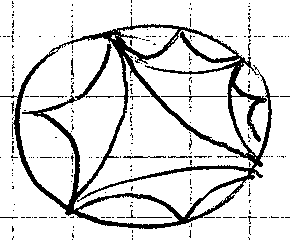
\includegraphics[width=\linewidth]{figures/gelfand-p001449-circle-diagram-original.png}
\par\smallskip{\footnotesize Original manuscript diagram: GELFAND-P001449\par}
\end{minipage}\hfill
\begin{minipage}[c]{0.48\linewidth}\centering
\resizebox{\linewidth}{!}{% Partial stroke comparison: nearby right-hand endings are not identified as one vertex.
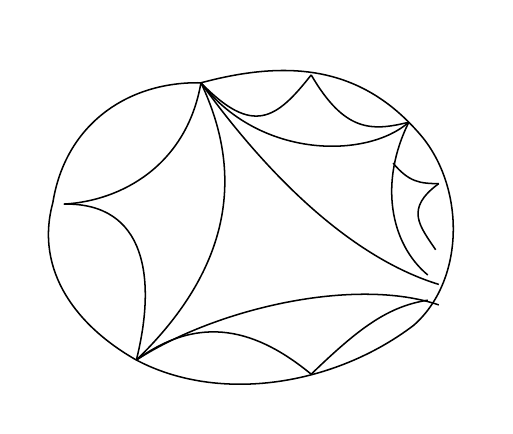
\begin{tikzpicture}[x=0.02cm,y=-0.02cm,line width=0.55pt]
\path[use as bounding box] (0,0) rectangle (290,240);
\draw (110,35)..controls(64,34)and(24,61)..(16,111)
 ..controls(4,155)and(32,190)..(69,211)
 ..controls(122,239)and(195,227)..(245,189)
 ..controls(277,161)and(278,104)..(251,70)
 ..controls(213,24)and(166,20)..(110,35);
\draw (110,35)..controls(139,96)and(127,155)..(69,211);
\draw (110,35)..controls(157,100)and(209,147)..(261,163);
\draw (69,211)..controls(120,178)and(208,158)..(261,176);
\draw (69,211)..controls(110,181)and(146,192)..(180,220);
\draw (180,220)..controls(211,190)and(229,177)..(254,173);
\draw (110,35)..controls(143,69)and(158,58)..(180,30);
\draw (180,30)..controls(201,66)and(218,66)..(242,60);
\draw (110,35)..controls(148,84)and(216,83)..(242,60);
\draw (242,60)..controls(223,98)and(230,137)..(254,157);
\draw (110,35)..controls(101,87)and(60,110)..(23,112);
\draw (23,112)..controls(75,111)and(82,159)..(69,211);
\draw (232,86)..controls(242,98)and(249,99)..(261,99);
\draw (261,99)..controls(239,115)and(249,126)..(259,141);
\end{tikzpicture}
}
\par\smallskip{\footnotesize Partial recreation of visible strokes; unresolved joins and labels remain explicit.\par}
\end{minipage}\par\medskip


How should these regions be parametrized?
\begin{equation*}
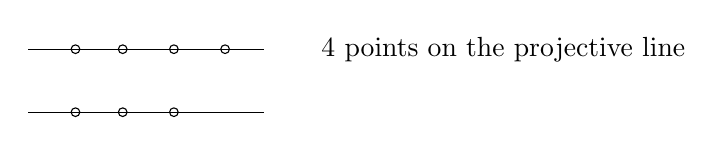
\begin{tikzpicture}
\draw (0,0)--(3,0);
\draw (0.6,0) circle (0.055);
\draw (1.2,0) circle (0.055);
\draw (1.85,0) circle (0.055);
\draw (2.5,0) circle (0.055);
\node[anchor=west] at (3.6,0) {4 points on the projective line};
\draw (0,-0.8)--(3,-0.8);
\draw (0.6,-0.8) circle (0.055);
\draw (1.2,-0.8) circle (0.055);
\draw (1.85,-0.8) circle (0.055);
\end{tikzpicture}
\end{equation*}
Strata of the Siegel domain $\Rightarrow$ configurations of lines in $\mathbb{R}\mathbb{P}^{2}$.

\underline{B.}

On MacPherson's work (on his work with Gelfand and Vilonen(?))

Perverse sheaves?

A perverse sheaf corresponds to problems in linear algebra that describe it completely,
but it is unclear how to single out the perverse sheaves.

\EnglishSourceFrame{GELFAND-P001450}{unlabelled}
$X$ is a complex manifold (smooth)

\underline{Constructible sheaf}

A stratification $\{X_i\}$ is given [above $X_i$, with a leader line: open];
a sheaf $\mathcal{F}$ on $X$ is called constructible
[inserted below this word: with respect to it]
if $\mathcal{F}|_{X_i}$ is a locally constant sheaf of finite-dimensional vector spaces

(locally: with respect to the usual topology)

\underline{Constructible complexes of sheaves}
\begin{equation*}
\ldots\longrightarrow\mathcal{F}^{-1}
\longrightarrow\mathcal{F}^{0}
\longrightarrow\mathcal{F}^{1}
\longrightarrow\mathcal{F}^{2}\longrightarrow\ldots \tag{1}
\end{equation*}
A complex of sheaves is called constructible if all the sheaves
$H^{i}(\mathcal{F}^{\bullet})$ are constructible.

(There are no conditions on $\mathcal{F}^{i}$!)

\underline{Singular support} of a sheaf or complex

$\mathcal{F}^{\bullet}$ is a constructible complex.
\begin{equation*}
SS(\mathcal{F})\subset T^{*}X \tag{2}
\end{equation*}
[Below $SS(\mathcal{F})$: subset]
is defined as follows.

Let $\nu\in T_x^{*}X$, $\nu\ne0$.
\EnglishUnclear{GELFAND-P001450}{covector-letter}{Covector letter: $\nu$ / $v$.}

(3) \underline{Definition.}
\begin{equation*}
\nu\notin SS(\mathcal{F})\ \Longleftrightarrow
\end{equation*}
[After the sign, inserted above the line: if]
one chooses a small neighbourhood $U\ni x$ and a holomorphic function $f$ on $U$
such that $df_x=\nu$, $f(x)=0$, then for $\forall$ points close to $0$,
$\varepsilon\in\mathbb{C}$,
\begin{equation*}
H^{*}\bigl(U,f^{-1}(\varepsilon);\mathcal{F}\bigr)=0. \tag{4}
\end{equation*}
[Below $f^{-1}(\varepsilon)$, added: $\cap\,U$.]

(relative cohomology groups modulo the fibre)

(more precisely, one must pass to the direct limit)

([Crossed out: \EnglishUnclear{GELFAND-P001450}{cycles-deletion}{appear. / illegible}]
$\ne0\ \Longleftrightarrow$ the appearance of vanishing cycles)

(4) does not depend on the choice of $f$

The zero section?

Add the zero section if $\mathcal{F}^{\bullet}$ is a nonzero complex.

$\mathcal{F}^{\bullet}$ is zero
$\Rightarrow SS(\mathcal{F}^{\bullet})\overset{\mathrm{df}}{=}\varnothing$.

\EnglishSourceFrame{GELFAND-P001451}{39}
(5) \underline{Theorem.}
$SS(\mathcal{F})$ is a conic Lagrangian subset

(an analytic subset whose nonsingular points are Lagrangian in the usual sense
[crossed-out sign: \EnglishUnclear{GELFAND-P001451}{sense-correction}{a closing parenthesis / an illegible sign}];
an equivalent condition is involutivity of the ideal)

Structure: a union of irreducible components (finitely many)

(6) \underline{Lemma.}
If $Y\subset T^{*}X$ is an irreducible conic Lagrangian subset, then
\begin{equation*}
Y=N^{*}Z\qquad
\text{for some irreducible }Z\subset X. \tag{7}
\end{equation*}
(the conormal bundle)

(then $Z=\pi(Y)$, $\pi:T^{*}X\longrightarrow X$)

Here $N^{*}Z$ is understood
[crossed out: \EnglishUnclear{GELFAND-P001451}{closure-deletion}{illegible}]
as the Zariski closure of
$N^{*}(\text{sm. part of }Z)$.
[After the opening parenthesis, crossed out:
\EnglishUnclear{GELFAND-P001451}{smooth-deletion}{an illegible sign}.]

[Crossed out before the heading:
\EnglishUnclear{GELFAND-P001451}{definition-deletion}{Perverse\ldots / illegible}.]

(8) \underline{Definition.}
Let a conic Lagrangian subset $Y\subset T^{*}X$ be given,
and let $f$ be a holomorphic function on $X$.

$f$ is called Morse with respect to $Y$ if it has the following property:

$df(X)$ (a Lagrangian subset (not conic!)) is transverse to $Y$,
\EnglishUnclear{GELFAND-P001451}{morse-bracket}{Before the explanation: a parenthesis with a short horizontal stroke.}

i.e. $df(X)$ intersects $Y$ only at smooth points and the intersection is transverse.

\underline{Examples.}

1. $Y=X$ is the zero section.

Then the Morse property of $f$ with respect to $Y$ = the Morse property in the usual sense.

2. $Y$ = the conormal to $Z$, $Y=N^{*}Z$, $Z$ is a smooth manifold.

Then the Morse property means that [crossed out: two]
\EnglishUnclear{GELFAND-P001451}{condition-ending}{condition / conditions} hold.

[The designation “a)” is crossed out.]
$g=f|_Z$ is a Morse function (in the usual sense).

[The following two lines are boxed and crossed out by two diagonals:]
\begin{equation*}
\text{b)}\quad dg(z)=0\ \Rightarrow\ df(z)\ne0.\qquad (?)
\end{equation*}
(If $Y$ contains the zero section, this is true)

\EnglishSourceFrame{GELFAND-P001452}{unlabelled}
(9) \underline{Definition.}
Let $\mathcal{F}^{\bullet}$ be a constructible complex; consider
$SS(\mathcal{F}^{\bullet})$, let $f$ be Morse with respect to
$SS(\mathcal{F}^{\bullet})$, and let $x$ be a critical point with respect to
$SS(\mathcal{F}^{\bullet})$
$\bigl(\overset{\mathrm{df}}{\Longleftrightarrow}
df(x)\in SS(\mathcal{F}^{\bullet})\bigr)$.
Then
\begin{equation*}
H^{*}\bigl(U,f^{-1}(\varepsilon);\mathcal{F}\bigr)\ne0.
\end{equation*}
The complex $\mathcal{F}$ is called a perverse sheaf
if all such groups occur in only one degree
(e.g. 0) [crossed out: \EnglishUnclear{GELFAND-P001452}{definition-deletion}{if / illegible}], i.e. if
\begin{equation*}
H^{j}\bigl(U,f^{-1}(\varepsilon);\mathcal{F}\bigr)=0
\quad\text{for }j\ne0. \tag{10}
\end{equation*}
(vanishing cycles exist only in the 1st degree)
\EnglishUnclear{GELFAND-P001452}{vanishing-degree}{The source has “in the 1st degree”.}

\underline{Examples.}
a. $\mathbb{C}_{x_0}$ is a perverse sheaf.
[Below the notation: concentrated at a point.]
(the stalk is $\mathbb{C}$ at $x_0$, $0$ on the complement)

b. $\mathbb{C}_X[n]$, the constant sheaf on $X$
(with a grading shift), is a perverse sheaf.
\begin{equation*}
n=\dim_{\mathbb{C}}X.
\end{equation*}
c. $Z\subset X$ [with a leader line: a smooth submanifold]
\begin{equation*}
\mathbb{C}_Z[\dim Z]
\end{equation*}
[Below the notation:]
the constant sheaf on $Z$, extended by zero outside $Z$.

(or: a shift of the Goresky--MacPherson complex)

\underline{Remark} (approximate).
The strata with respect to which the sheaf $\mathcal{F}$ is constructible
are the projections to the base of the irreducible components of its $SS(\mathcal{F})$.

\underline{Construction 1.}
Let $\mathcal{F}$ be a perverse sheaf.
Construct a local system [inserted: $\Phi(\mathcal{F})$]
on the smooth points of its $SS(\mathcal{F})$.

Let [crossed out: \EnglishUnclear{GELFAND-P001452}{point-deletion}{an illegible sign}]
$z$ be a smooth point of $SS(\mathcal{F})$.
Then
\begin{equation*}
\Phi(\mathcal{F})=
H^{0}\bigl(U,f^{-1}(\varepsilon),\mathcal{F}\bigr),
\qquad df(\pi(z))=z. \tag{11}
\end{equation*}
(nothing depends on the choice of $f$)

\underline{Next time: in 2 weeks.}

\EnglishSourceFrame{GELFAND-P001453}{unlabelled}
\EnglishUnclear{GELFAND-P001453}{page-label}{Leaf number: 42 or 48.}

\underline{11/IV--88}\quad \underline{Gelfand's seminar}

\underline{\underline{D.B. Fuchs.}}\quad
\underline{\underline{The $4$-colour problem.}}\quad
(Appel; Haken)

\underline{Definition.} A configuration is a triangulation of a disk.

[Crossed out on the right: “--- a subdivision of a sphere
(\EnglishUnclear{GELFAND-P001453}{top-cancelled-definition}{disk?; plane [abbr.]?})
(a triangulation)”.]

\EnglishSourceFigure{GELFAND-P001453}{diagram-disk}{Drawing to the right of the definition: a polygonal outline with internal edges. In several places the strokes do not meet; the exact joins of the internal edges require checking against the original.}

\par\medskip\noindent
\begin{minipage}[c]{0.48\linewidth}\centering
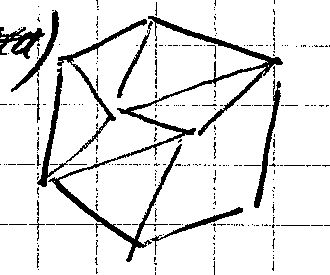
\includegraphics[width=\linewidth]{figures/gelfand-p001453-diagram-disk-original.png}
\par\smallskip{\footnotesize Original manuscript diagram: GELFAND-P001453\par}
\end{minipage}\hfill
\begin{minipage}[c]{0.48\linewidth}\centering
\resizebox{\linewidth}{!}{% Partial trace in crop-pixel coordinates. All visible gaps remain unjoined.
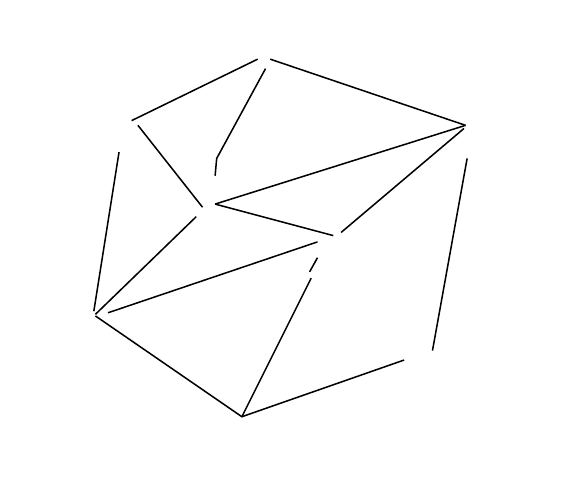
\begin{tikzpicture}[x=0.02cm,y=-0.02cm,line width=0.55pt]
\path[use as bounding box] (0,0) rectangle (330,275);
\draw (66,59)--(146,20);
\draw (154,20)--(278,62);
\draw (279,83)--(257,205);
\draw (239,211)--(136,247)--(43,183);
\draw (42,180)--(58,79);
\draw (70,62)--(111,114);
\draw (107,120)--(43,182);
\draw (119,112)--(194,132);
\draw (199,130)--(277,64);
\draw (119,112)--(278,62);
\draw (136,247)--(180,159);
\draw (184,146)--(179,155);
\draw (151,26)--(120,83)--(119,94);
\draw (51,181)--(184,136);
\end{tikzpicture}
}
\par\smallskip{\footnotesize Partial recreation of visible strokes; unresolved joins and labels remain explicit.\par}
\end{minipage}\par\medskip


(1) One must prove that the vertices can be coloured with 4 colours
[\EnglishUnclear{GELFAND-P001453}{line-one-cancellation}{a short cancelled fragment is illegible}]
so that adjacent vertices have different colours.

[Small annotation:] (this is the dual problem to colouring faces; therefore
\EnglishUnclear{GELFAND-P001453}{parenthetical-tail}{only another?; only others?}

(2) A set of configurations is called \underline{unavoidable}
if one of them occurs in every triangulation.

(3) A configuration is called \underline{reducible} if it cannot occur in
a triangulation of a sphere that cannot be coloured with 4 colours
and has the least number of vertices among such triangulations.

\underline{Reducible triangulation $K$:}
[crossed out: \EnglishUnclear{GELFAND-P001453}{reducibility-cancelled-if}{if?}; inserted above: “let”]
there is a triangulation $T\supset K$, and it is known
that $\forall$ configurations
[\EnglishUnclear{GELFAND-P001453}{reducibility-cancelled-word}{a cancelled word is illegible}]
with fewer vertices (than $T$) can be coloured with 4 colours;
then $T$ can be coloured too.

Induction on the number of vertices $N$.

\underline{Suppose it has already been proved for $N-1$ vertices.}

A configuration [crossed out:
\EnglishUnclear{GELFAND-P001453}{induction-cancelled-word}{this?}] $K$
is called \underline{reducible} if
[inserted above: “from”] its occurrence in $T$ with
$|T|=N$ implies that $T$ can be coloured.

[Crossed out: “Example.”]

The main idea is to combine definitions (2) and (3).

[Crossed out: “It is necessary”; inserted above: “It is sufficient”]
to construct an unavoidable set of reducible configurations.

(4) \underline{Example.}

\begin{center}
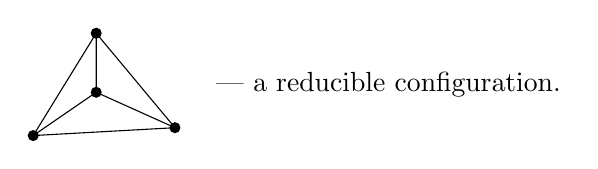
\begin{tikzpicture}[x=1cm,y=1cm]
\draw (0,0)--(.8,1.3)--(1.8,.1)--cycle;
\draw (.8,.55)--(0,0) (.8,.55)--(.8,1.3) (.8,.55)--(1.8,.1);
\fill (0,0) circle (2pt);
\fill (.8,1.3) circle (2pt);
\fill (1.8,.1) circle (2pt);
\fill (.8,.55) circle (2pt);
\node[anchor=west] at (2.2,.65) {--- a reducible configuration.};
\end{tikzpicture}
\end{center}

\begin{center}
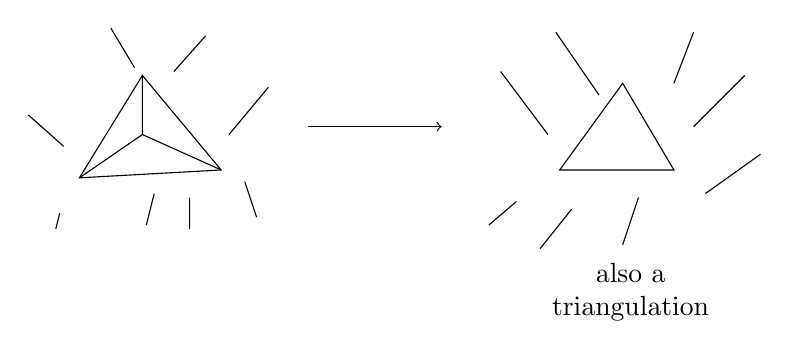
\begin{tikzpicture}[x=1cm,y=1cm]
\draw (0,0)--(.8,1.3)--(1.8,.1)--cycle;
\draw (.8,.55)--(0,0) (.8,.55)--(.8,1.3) (.8,.55)--(1.8,.1);
\draw (-.65,.8)--(-.2,.4) (.4,1.9)--(.7,1.4)
      (1.6,1.8)--(1.2,1.35) (2.4,1.15)--(1.9,.55)
      (-.3,-.65)--(-.25,-.45) (.85,-.6)--(.95,-.2)
      (1.4,-.65)--(1.4,-.25) (2.25,-.5)--(2.1,-.05);
\draw[->] (2.9,.65)--(4.6,.65);
\draw (6.1,.1)--(6.9,1.2)--(7.55,.1)--cycle;
\draw (5.35,1.35)--(5.95,.55) (6.05,1.85)--(6.6,1.05)
      (7.8,1.85)--(7.55,1.2) (8.45,1.3)--(7.8,.65)
      (8.65,.3)--(7.95,-.2) (6.9,-.85)--(7.1,-.25)
      (5.85,-.9)--(6.25,-.4) (5.2,-.6)--(5.55,-.3);
\node[align=center] at (7,-1.45) {also a\\triangulation};
\end{tikzpicture}
\end{center}

\EnglishSourceFrame{GELFAND-P001454}{unlabelled}
\underline{I.M.G.} Everything should be devised using the simplest examples.
(I. Bernstein learned this from I.M.G.)

I.M.G. devised the whole theory of spherical functions from the formula
\begin{equation*}
\cos(\alpha+\beta)+\cos(\alpha-\beta)=2\cos\alpha\cdot\cos\beta.
\end{equation*}
On $\mathbb R$, consider the group generated by translations and reflections.

[Above the following heading, crossed out:
\EnglishUnclear{GELFAND-P001454}{cancelled-theorem-heading}{Assert.?}]

(5) \underline{Theorem}
\begin{center}
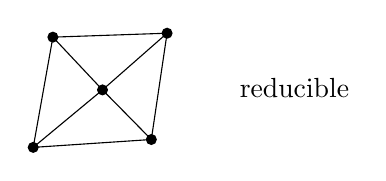
\begin{tikzpicture}[x=1cm,y=1cm]
\draw (0,0)--(.25,1.4)--(1.7,1.45)--(1.5,.1)--cycle;
\draw (0,0)--(.88,.73)--(1.7,1.45);
\draw (.25,1.4)--(.88,.73)--(1.5,.1);
\fill (0,0) circle (2pt);
\fill (.25,1.4) circle (2pt);
\fill (1.7,1.45) circle (2pt);
\fill (1.5,.1) circle (2pt);
\fill (.88,.73) circle (2pt);
\node[anchor=west] at (2.5,.75) {reducible};
\end{tikzpicture}
\end{center}

(Kempe; $\sim 100$ years ago)

Replace it with

(6)
\begin{center}
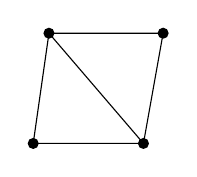
\begin{tikzpicture}[x=1cm,y=1cm]
\draw (0,0)--(.2,1.4)--(1.65,1.4)--(1.4,0)--cycle;
\draw (.2,1.4)--(1.4,0);
\fill (0,0) circle (2pt);
\fill (.2,1.4) circle (2pt);
\fill (1.65,1.4) circle (2pt);
\fill (1.4,0) circle (2pt);
\end{tikzpicture}
\end{center}
and colour the resulting triangulation.

(*) If some of the four have the same colour, colour the centre with a free colour.
\begin{center}
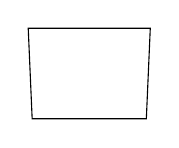
\begin{tikzpicture}[x=1cm,y=1cm]
\draw (0,0)--(-.05,1.15)--(1.5,1.15)--(1.45,0)--cycle;
\end{tikzpicture}
\end{center}

It remains to consider the case

(7)
\begin{center}
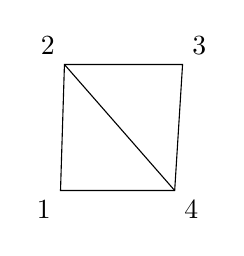
\begin{tikzpicture}[x=1cm,y=1cm]
\draw (0,0)--(.05,1.6)--(1.55,1.6)--(1.45,0)--cycle;
\draw (.05,1.6)--(1.45,0);
\node[below left] at (0,0) {$1$};
\node[above left] at (.05,1.6) {$2$};
\node[above right] at (1.55,1.6) {$3$};
\node[below right] at (1.45,0) {$4$};
\end{tikzpicture}
\end{center}

Consider the subset $K$ consisting of vertices coloured 1 and 3 and edges
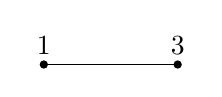
\begin{tikzpicture}[baseline=0pt,x=1cm,y=1cm]
\draw (0,0)--(1.7,0);
\fill (0,0) circle (1.5pt);
\fill (1.7,0) circle (1.5pt);
\node[above] at (0,0) {$1$};
\node[above] at (1.7,0) {$3$};
\end{tikzpicture}

(8) 1 may a) be connected to 3 in $K$

or b) not be connected.

Case b): in this connected component of vertex 1,
interchange 1 and 3 and reduce to the preceding case (*).

(9)
\EnglishSourceFigure{GELFAND-P001454}{diagram-path}{A square with a diagonal from the upper-left to the lower-right vertex; corner labels are 1 at lower left, 2 at upper left, 3 at upper right, and 4 at lower right. Outside, below and to the right, a line has a continuous initial part and separate continuation strokes; its lower bends are labelled 3, 1 and a corrected digit resembling 3. The exact last label and joins of the broken continuation require checking against the original.}

\par\medskip\noindent
\begin{minipage}[c]{0.48\linewidth}\centering
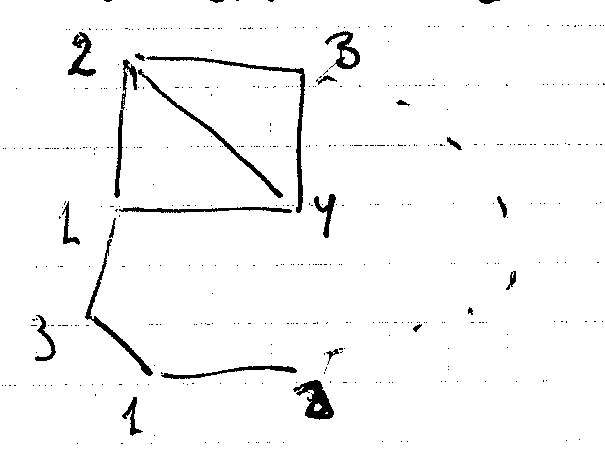
\includegraphics[width=\linewidth]{figures/gelfand-p001454-diagram-path-original.png}
\par\smallskip{\footnotesize Original manuscript diagram: GELFAND-P001454\par}
\end{minipage}\hfill
\begin{minipage}[c]{0.48\linewidth}\centering
\resizebox{\linewidth}{!}{% Partial source-stroke trace. The right-hand continuation stays separate.
% The bracketed bottom digit is an uncertainty marker, not a new decipherment.
\begin{tikzpicture}[x=0.01cm,y=-0.01cm,line width=0.55pt]
\path[use as bounding box] (0,0) rectangle (605,460);
\draw (118,194)--(123,68);
\draw (136,58)--(302,71)--(300,210);
\draw (117,210)--(291,210);
\draw (135,75)--(281,195);
\draw (113,242)--(87,316)--(148,373);
\draw (163,376)..controls(207,379)and(247,362)..(295,371);
\draw (398,104)--(407,105);
\draw (447,139)--(461,150);
\draw (500,198)--(506,214);
\draw (514,272)--(511,286);
\draw (470,307)--(473,314);
\draw (415,328)--(423,321);
\node at (76,55) {$2$};\node at (345,46) {$3$};
\node at (67,230) {$1$};\node at (325,216) {$4$};
\node at (45,340) {$3$};\node at (132,418) {$1$};
\node at (330,410) {$[3/8\,?]$};
\end{tikzpicture}
}
\par\smallskip{\footnotesize Partial recreation of visible strokes; unresolved joins and labels remain explicit.\par}
\end{minipage}\par\medskip


[To the right of the drawing:]

Suppose case 8a) holds.

Then there is no path from 2 to 4
with [crossed out: \EnglishUnclear{GELFAND-P001454}{cancelled-before-two}{a cancelled fragment is illegible}] 2 and 4.

\EnglishSourceFigure{GELFAND-P001454}{diagram-excluded-edge}{Two small drawings: a square with a diagonal and a separate sloping edge. The same looped exclusion mark is on the diagonal and on the separate edge. The caption to the right reads: “--- we do not count this edge”. The exact form of the looped mark requires checking against the original.}

\par\medskip\noindent
\begin{minipage}[c]{0.48\linewidth}\centering
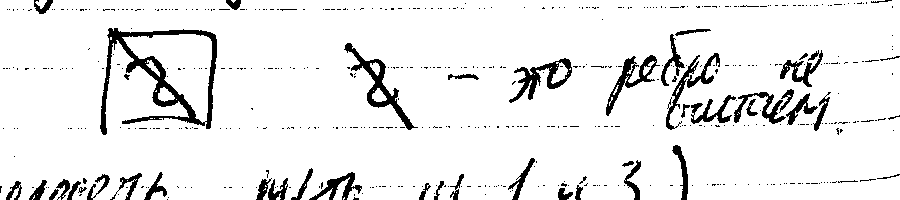
\includegraphics[width=\linewidth]{figures/gelfand-p001454-diagram-excluded-edge-original.png}
\par\smallskip{\footnotesize Original manuscript diagram: GELFAND-P001454\par}
\end{minipage}\hfill
\begin{minipage}[c]{0.48\linewidth}\centering
\resizebox{\linewidth}{!}{\def\ExcludedEdgeCaption{We do not count this edge.}
% Literal two-loop edge annotation; it adds no graph vertex.
\begin{tikzpicture}[x=0.01cm,y=-0.01cm,line width=0.55pt]
\path[use as bounding box] (0,0) rectangle (900,175);
\draw (104,130)--(110,33)--(214,32)--(210,126);
\draw (121,124)..controls(160,111)and(187,114)..(201,122);
\draw (114,36)--(197,118);
\draw (129,73)..controls(145,48)and(161,60)..(160,76)
 ..controls(158,89)and(140,100)..(155,104)
 ..controls(172,108)and(180,97)..(178,91);
\draw (346,47)--(410,127);
\draw (346,77)..controls(366,49)and(383,64)..(381,78)
 ..controls(379,94)and(357,109)..(372,114)
 ..controls(389,118)and(402,105)..(399,97);
\node[anchor=west,text width=3.7cm,align=left] at (455,80) {\ExcludedEdgeCaption};
\end{tikzpicture}
}
\par\smallskip{\footnotesize Partial recreation of visible strokes; unresolved joins and labels remain explicit.\par}
\end{minipage}\par\medskip


(because it cannot cross the path of 1 and 3)

and then reduce to 8b) again.

